% =============================================================================
% presentacion.tex
% Presentación para la defensa del Trabajo de Fin de Grado (TFG)
% Título: Estudio de mejora de la imagen PET con Itrio-86 mediante simulación Monte Carlo y técnicas de multiplexado
% Autor: Guillermo Gutiérrez Caracuel
% Compile con: lualatex presentacion.tex
% =============================================================================
\documentclass[aspectratio=169]{beamer}
\usepackage{beamerthememidcenturymodern}
\usepackage[spanish, es-tabla]{babel}
\usepackage[version=4]{mhchem}
\usepackage{siunitx}
\usepackage{booktabs}
\usepackage{xspace}
\usepackage{listings}
\usepackage{tikz}
\usetikzlibrary{positioning, chains, arrows, shapes, babel}

% --- Custom Command Definitions ---
\newcommand{\yochoseis}{\ce{^{86}Y}\xspace}
\newcommand{\ynuevecero}{\ce{^{90}Y}\xspace}
\newcommand{\fdiezocho}{\ce{^{18}F}\xspace}
\newcommand{\conce}{\ce{^{11}C}\xspace}
\newcommand{\penred}{\texttt{penRed}\xspace}
\newcommand{\ingles}[1]{\textit{#1}\xspace}

% --- Theme selection (Kraft is terracotta, warm tones) ---
\mcmTheme{Kraft}

% --- Metadata ---
\title{Mejora de la imagen PET con Itrio-86}
\subtitle{Simulación Monte Carlo y técnicas de multiplexado}
\author[Guillermo Gutiérrez Caracuel]{Guillermo Gutiérrez Caracuel \\ \small Tutor: Vicent Giménez Alventosa}
\institute{Escuela Técnica Superior de Ingeniería Industrial (ETSII) \\ Universitat Politècnica de València}
\date{Defensa de Trabajo de Fin de Grado — 12 de junio de 2026}

% Graphicspath to search in figures and logos
\graphicspath{
  {./logos/}
  {../figuras/}
  {../logos/}
}

\titlegraphic{
  \begin{minipage}{0.65\linewidth}
    \centering
    
\includegraphics[height=0.9cm]{UPV_horitzontal_color.jpg}
    \hspace{0.4cm}
    
\includegraphics[height=0.9cm]{ETSII_vectorial_horizontal.pdf}
    \hspace{0.4cm}
    
\includegraphics[height=0.8cm]{logo_bruker.pdf}
  \end{minipage}
}

% --- Automatic section/subsection pages ---
\AtBeginSection[]{%
  \begin{frame}[plain]
    \sectionpage
  \end{frame}
}

\begin{document}

% =====================================================================
% DIAPOSITIVA DE PORTADA
% =====================================================================
\begin{frame}[plain]
    \titlepage
\end{frame}

% =====================================================================
% ALINEACIÓN CON LOS ODS
% =====================================================================
\begin{frame}{Alineación con los ODS}
    \begin{columns}[T]
        \begin{column}{0.48\textwidth}
            \begin{block}{Relación Directa (Grado Alto)}
                \begin{itemize}
                    \item \textbf{ODS 3:} Salud y bienestar
                    \item \textbf{ODS 9:} Industria, innovación e infraestructura
                \end{itemize}
            \end{block}
        \end{column}
        \begin{column}{0.48\textwidth}
            \begin{exampleblock}{Relación Indirecta (Grado Medio)}
                \begin{itemize}
                    \item \textbf{ODS 4:} Educación de calidad
                    \item \textbf{ODS 17:} Alianzas para lograr los objetivos
                \end{itemize}
            \end{exampleblock}
        \end{column}
    \end{columns}
    \vspace{0.4cm}
    % NOTA DEL PONENTE: Este trabajo se alinea de forma directa con los Objetivos de Desarrollo Sostenible de la Agenda 2030, concretamente con el ODS 3 (Salud y bienestar) al contribuir al avance de la teranosis y la medicina oncológica personalizada, y con el ODS 9 (Industria, innovación e infraestructura) mediante la innovación tecnológica preclínica en colaboración con Bruker. De manera indirecta, también se vincula con los ODS 4 (Educación de calidad) y ODS 17 (Alianzas).
\end{frame}

% =====================================================================
% ESTRUCTURA DE LA PRESENTACIÓN
% =====================================================================
\begin{frame}{Estructura de la Presentación}
    \begin{columns}[T]
        \begin{column}{0.9\textwidth}
            \begin{block}{Índice de Contenidos}
                \tableofcontents[hideallsubsections]
            \end{block}
        \end{column}
    \end{columns}
\end{frame}

% =====================================================================
% SECCIÓN 1: INTRODUCCIÓN Y OBJETIVOS
% =====================================================================
\section{Introducción y Objetivos}
% --- Diapositiva 3 ---
\begin{frame}{El Paradigma de la Teranosis}
    \begin{columns}[T]
        \begin{column}{0.62\textwidth}
            \begin{block}{Fundamentos de la Teranosis}
                \begin{itemize}
                    \item \alert{Terapia + diagnóstico:} \textit{«Vemos lo que tratamos y tratamos lo que vemos»}.
                    \item \textbf{El par teranóstico verdadero (\yochoseis / \ynuevecero):}
                    \begin{itemize}
                        \item Mismo elemento, biodistribución 100\% idéntica.
                        \item \textbf{\yochoseis:} Emisor $\beta^+$ para el escáner \alert{PET} previo (diagnóstico/planificación).
                        \item \textbf{\ynuevecero:} Emisor $\beta^-$ para radioterapia dirigida (destrucción).
                    \end{itemize}
                \end{itemize}
            \end{block}
        \end{column}
        \begin{column}{0.32\textwidth}
            \centering
            \vspace{0.1cm}
            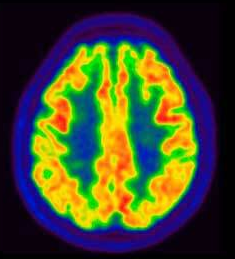
\includegraphics[height=4cm,keepaspectratio]{ejemploPet.png}
            \vskip0.1cm
            {\scriptsize\color{mcmBlack!65} Figura 1. Imagen PET cerebral (diagnóstico por imagen funcional).\par}
            \vspace{0.05cm}
            {\tiny\color{mcmBlack!40} [Fuente: \href{https://www.centremedicalomar.es/tienda/diagnostico-imagen/pet-tac/pet-tac-cerebral-con-fdg-en-reus/}{\underline{centremedicalomar.es}}]\par}
        \end{column}
    \end{columns}
    \vspace{0.2cm}
    % NOTA DEL PONENTE: Buenos días. Comenzamos la presentación de mi TFG. La teranosis en medicina nuclear funciona uniendo un isótopo a una molécula portadora, un vector biológico con alta afinidad por los receptores del tumor. La clave está en la carga. El par Y-86/Y-90 es lo que llamamos un par teranóstico verdadero. Como son el mismo elemento, la química es idéntica y el cuerpo no los distingue. Primero inyectamos la molécula con Y-86, el "explorador" emisor de positrones, para hacer un PET —que es una tomografía por emisión de positrones, una técnica de diagnóstico por imagen funcional de medicina nuclear— y planificar. Días después, inyectamos la misma molécula con Y-90, el "tratamiento", para hacer radioterapia local. El Y-86 nos da un mapa de diagnóstico y biodistribución perfecto de dónde irá la radioterapia.
\end{frame}

% --- Diapositiva 3b: Esquemas de desintegración ---
\begin{frame}{Esquemas de Desintegración}
    \centering
    \begin{columns}[c]
        \begin{column}{0.48\textwidth}
            \centering
            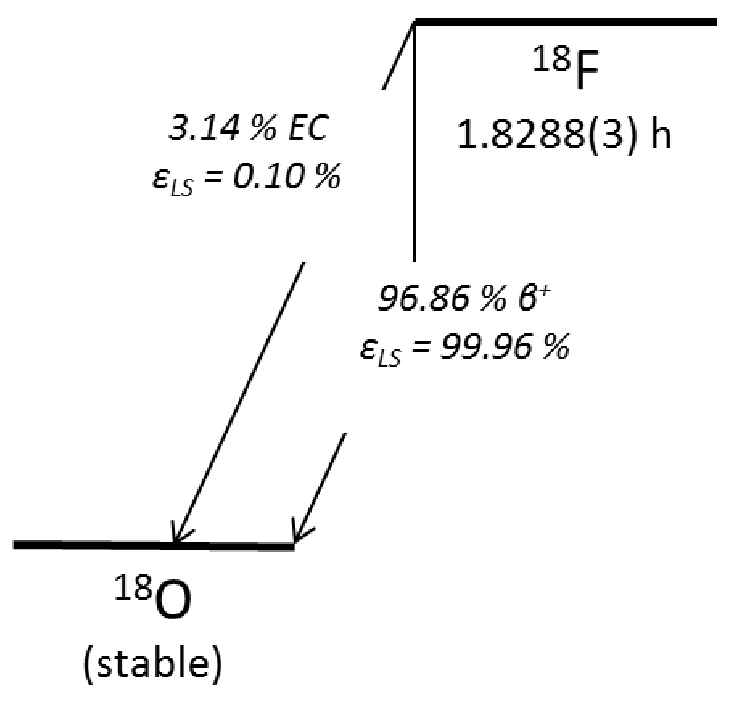
\includegraphics[height=6.0cm,keepaspectratio]{esquemaf18.png}
            \vskip0.15cm
            {\scriptsize\color{mcmBlack!65} Figura 2. Esquema de desintegración del \fdiezocho (emisor $\beta^+$ puro).\par}
            \vspace{0.1cm}
            {\tiny\color{mcmBlack!40} [Bergeron et al., 2014]\par}
        \end{column}
        \begin{column}{0.48\textwidth}
            \centering
            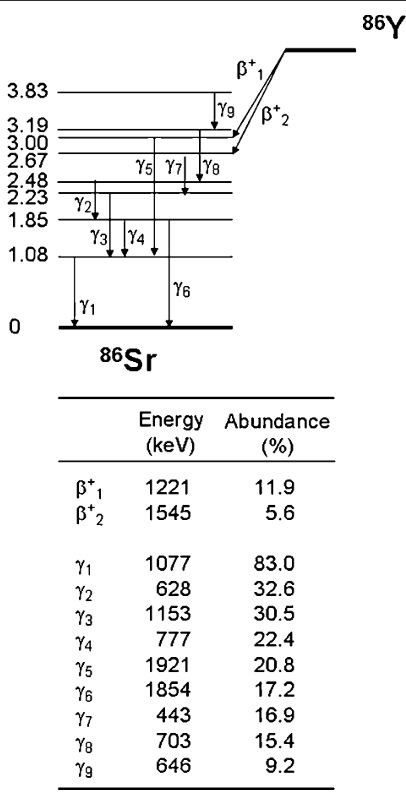
\includegraphics[height=6.0cm,keepaspectratio]{esquemaY86.png}
            \vskip0.15cm
            {\scriptsize\color{mcmBlack!65} Figura 3. Esquema de desintegración del \yochoseis (emisor complejo con prompt gammas).\par}
            \vspace{0.1cm}
            {\tiny\color{mcmBlack!40} [Adaptado de Lubberink y Herzog, 2011]\par}
        \end{column}
    \end{columns}
    % NOTA DEL PONENTE: A la izquierda vemos el esquema de desintegración del Flúor-18, un emisor beta-positivo puro que decae directamente al estado base. A la derecha, el esquema del Itrio-86 revela la raíz física de nuestro problema: este isótopo no decae al estado fundamental, sino a múltiples estados energéticos excitados del Estroncio-86 (Sr-86). Para alcanzar la estabilidad, el núcleo hijo de Estroncio se desexcita emitiendo casi instantáneamente esa compleja cascada de fotones o "prompt gammas", que son la verdadera fuente de ruido en nuestra imagen PET.
\end{frame}

% --- Diapositiva 4 ---
\begin{frame}{El Problema Físico del Itrio-86}
    \begin{columns}[c]
        \begin{column}{0.54\textwidth}
            \begin{block}{El Desafío Físico del \yochoseis}
                \begin{itemize}
                    \item \textbf{Decaimiento sucio:} Emisión de \alert{gammas en cascada} (\ingles{prompt gammas}).
                    \item \textbf{Dispersión Compton:} Deposita energía en el rango de la ventana de detección (\SI{511}{\kilo\electronvolt}).
                    \item \textbf{Efecto:} Da lugar a \alert{coincidencias triples y espurias}.
                \end{itemize}
            \end{block}
        \end{column}
        \begin{column}{0.42\textwidth}
            \centering
            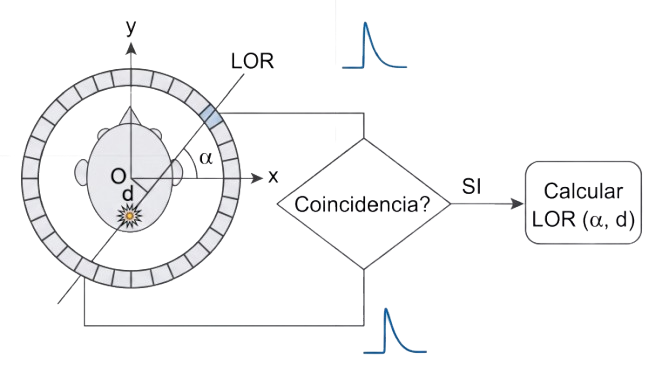
\includegraphics[height=3.6cm,keepaspectratio]{deteccion_coincidencia.png}
            \vskip0.1cm
            {\scriptsize\color{mcmBlack!65} Figura 4. Coincidencia PET estándar.\par}
        \end{column}
    \end{columns}
    % NOTA DEL PONENTE: Sin embargo, el Y-86 presenta graves desafíos físicos. Se le conoce como un isótopo "sucio" debido a que emite gammas rápidos en cascada. El de 1077 keV se emite en el 82.5% de los decaimientos, superando a los propios positrones. Estos gammas de alta energía interactúan Compton en el tejido y depositan energía que cae justo en la ventana de detección de 511 keV, contaminando la adquisición.
\end{frame}

% --- Diapositiva 5 ---
\begin{frame}{El Impacto en la Imagen: Coincidencias Espurias}
    \begin{columns}[T]
        \begin{column}{0.52\textwidth}
            \begin{alertblock}{Impacto de las Coincidencias Triples}
                \begin{itemize}
                    \item \textbf{Verdaderas:} Par de \SI{511}{\kilo\electronvolt} a $180^\circ$.
                    \item \textbf{Triples (\yochoseis):} Par PET detectado junto a un \alert{prompt gamma}.
                    \item \textbf{Degradación:} Falsean la línea de respuesta (LOR).
                    \item \textbf{Efecto:} Halo de fondo que colapsa el contraste (\textbf{CRC}).
                \end{itemize}
            \end{alertblock}
        \end{column}
        \begin{column}{0.44\textwidth}
            \centering
            \includegraphics[height=4.0cm,keepaspectratio]{triple_coincidence.png}
            \vskip0.1cm
            {\scriptsize\color{mcmBlack!65} Figura 5. Mecanismo de coincidencia triple (falsa doble) debido a la emisión simultánea de un prompt gamma.\par}
        \end{column}
    \end{columns}
    % NOTA DEL PONENTE: Aquí vemos el mecanismo de interferencia. Un PET estándar busca coincidencias dobles de 511 keV. Pero en el Y-86, al emitirse un prompt gamma simultáneamente, la electrónica puede registrar una coincidencia triple. Al no poder procesarla, el sistema genera líneas de respuesta erróneas o dobles falsas, provocando un halo de ruido masivo y reduciendo severamente el contraste de la imagen.
\end{frame}

% --- Diapositiva 6: Motivación Clínica mPET ---
\begin{frame}{Motivación Clínica: Multiplexado (mPET)}
    \begin{columns}[c]
        \begin{column}{0.50\textwidth}
            \begin{block}{El Cambio de Paradigma}
                \begin{itemize}
                    \item \textbf{De ruido a señal:} Usar los \ingles{prompt gammas} como \textbf{firma única} para discriminar isótopos.
                    \item \textbf{Correlación biológica:} Visión dinámica simultánea de dos procesos distintos.
                \end{itemize}
            \end{block}
            \begin{exampleblock}{Beneficio Hospitalario}
                \begin{itemize}
                    \item Una sesión PET en vez de 2.
                    \item \alert{Reducción de dosis:} Evita doble exposición de rayos X al no repetir escáner CT.
                \end{itemize}
            \end{exampleblock}
        \end{column}
        \begin{column}{0.48\textwidth}
            \centering
            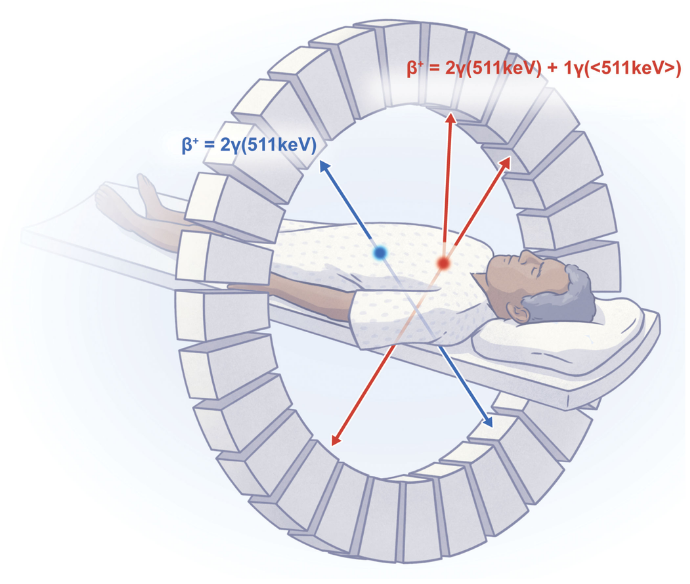
\includegraphics[width=\textwidth,keepaspectratio]{../figuras/multiplexing_ejemplo.png}
            \vskip0.1cm
            {\scriptsize\color{mcmBlack!65} Figura 6. Esquema de adquisición simultánea dual (mPET).\par}
            \vspace{0.2cm}
            \hfill {\tiny\color{mcmBlack!40} [Pratt et al., 2023]}
        \end{column}
    \end{columns}
    % NOTA DEL PONENTE: Además de la corrección, este trabajo explora una motivación innovadora: el cambio de paradigma hacia la imagen multiplexada. Planteamos usar los prompt gammas no como ruido, sino como una firma para distinguir eventos de un isótopo sucio frente a otro puro, abriendo la puerta a adquisiciones simultáneas duales o mPET. Esto ofrece una correlación espacio-temporal óptima para observar interacciones entre dos procesos biológicos. Clínicamente esto es vital: frente al PET convencional que requeriría dos sesiones, el multiplexado lo consolida en una sola. Esto no solo reduce drásticamente el tiempo de ocupación del escáner, sino que disminuye enormemente la dosis de radiación al paciente, ya que le ahorramos la exposición a la segunda tomografía computarizada (CT) que siempre es necesaria para la corrección de atenuación en cada sesión independiente.
\end{frame}

% --- Diapositiva 7 ---
\begin{frame}{Alcance y Objetivos del Proyecto}
    \begin{columns}[c]
        \begin{column}{0.54\textwidth}
            \begin{block}{Objetivo General}
                Optimizar la imagen PET de \yochoseis mediante simulación Monte Carlo de alta fidelidad y técnicas de multiplexado (\textbf{mPET}).
            \end{block}
            \begin{exampleblock}{Alcance Específico}
                \begin{itemize}\setlength{\itemsep}{0.6em}
                    \item \textbf{Modelado y Simulación}
                    \item \textbf{Software de Post-procesado}
                    \item \textbf{Estudio de Optimización}
                    \item \textbf{Prueba de Concepto (mPET)}
                \end{itemize}
            \end{exampleblock}
        \end{column}
        \begin{column}{0.42\textwidth}
            \centering
            \includegraphics[width=0.7\textwidth]{Si78--357.png}
            \vskip0.1cm
            {\scriptsize\color{mcmBlack!65} Figura 7. Fotografía Bruker PET/CT Si78.\par}
            \vspace{0.2cm}
            \hfill {\tiny\color{mcmBlack!40} [www.bruker.com]}
        \end{column}
    \end{columns}
    % NOTA DEL PONENTE: El alcance del proyecto abarca cuatro fases fundamentales. En primer lugar, el modelado en Blender y simulación en penRed del escáner preclínico Bruker Si78 y el fantoma Derenzo. En segundo lugar, el desarrollo de software de post-procesado en C++ para clasificar las coincidencias. En tercer lugar, el estudio de optimización de las ventanas energéticas y de coincidencia temporal. Y por último, la prueba de concepto de multiplexado mPET para la separación física y computacional de ambos trazadores.
\end{frame}

% =====================================================================
% SECCIÓN 2: METODOLOGÍA Y DESARROLLO
% =====================================================================
\section{Metodología y Desarrollo}

% --- Diapositiva 7 ---
\begin{frame}{Flujo de Trabajo Metodológico}
    \centering
    \begin{tikzpicture}[
            node distance=1cm and 0.8cm,
            box/.style={
                    draw=mcmPrimary,
                    thick,
                    fill=mcmPrimaryMuted!40,
                    text=mcmBlack,
                    font=\bfseries\scriptsize,
                    align=center,
                    minimum height=2cm,
                    text width=3.2cm,
                    rounded corners=3pt
                },
            arrow/.style={
                    ->,
                    >=stealth,
                    thick,
                    mcmPrimary
                }
        ]
        \node (blender) [box] {
\includegraphics[height=0.9cm]{logo_blender.png}\\[1mm] 1. Modelado 3D\\(Blender + plugin\\\penred)};
        \node (sim) [box, right=of blender] {
\includegraphics[height=0.9cm]{PenRed_color.png}\\[1mm] 2. Simulación MC\\(Monte Carlo\\\penred + PENNUC)};
        \node (post) [box, right=of sim] {
\includegraphics[height=0.9cm]{cpp_logo.png}\\[1mm] 3. Post-procesado\\(C++: singles a\\coincidencias LM)};

        % Segunda fila, bajando desde el nodo 3 y yendo hacia la izquierda
        \node (reco) [box, below=of post, yshift=-0.5cm] {
\includegraphics[height=0.6cm]{logo_bruker.pdf}\\[1mm] 4. Reconstrucción\\(Bruker RecoServer\\algoritmo MLEM)};
        \node (anal) [box, left=of reco] {5. Análisis / mPET\\(AMIDE y sustracción\\en Python)};

        \draw [arrow] (blender) -- (sim);
        \draw [arrow] (sim) -- (post);
        \draw [arrow] (post) -- (reco);
        \draw [arrow] (reco) -- (anal);
    \end{tikzpicture}
    % NOTA DEL PONENTE: Este diagrama representa nuestro flujo metodológico. Es un enfoque integral "in silico". Comenzamos modelando en Blender, simulamos en Quasar, post-procesamos las cuentas con nuestro algoritmo C++, reconstruimos con el software comercial RecoServer de la propia Bruker y finalmente analizamos las imágenes resultantes en AMIDE y un script de Python que implementa la sustracción.
\end{frame}

% --- Diapositiva 8 ---
\begin{frame}{Modelado Geométrico: Escáner y Fantoma}
    \begin{columns}[T]
        \begin{column}{0.54\textwidth}
            \begin{block}{Geometría en Blender}
                \begin{itemize}
                    \item \textbf{Bruker Si78:} Escáner octogonal preclínico con 3 anillos de detectores de LYSO ($48\times 48\times 10$\,mm).
                    \item \textbf{Fantoma Derenzo:} PMMA ($R=35$\,mm) con 6 sectores de varillas ($0.8$ a $2.5$\,mm) rellenas de actividad.
                \end{itemize}
            \end{block}
        \end{column}
        \begin{column}{0.42\textwidth}
            \centering
            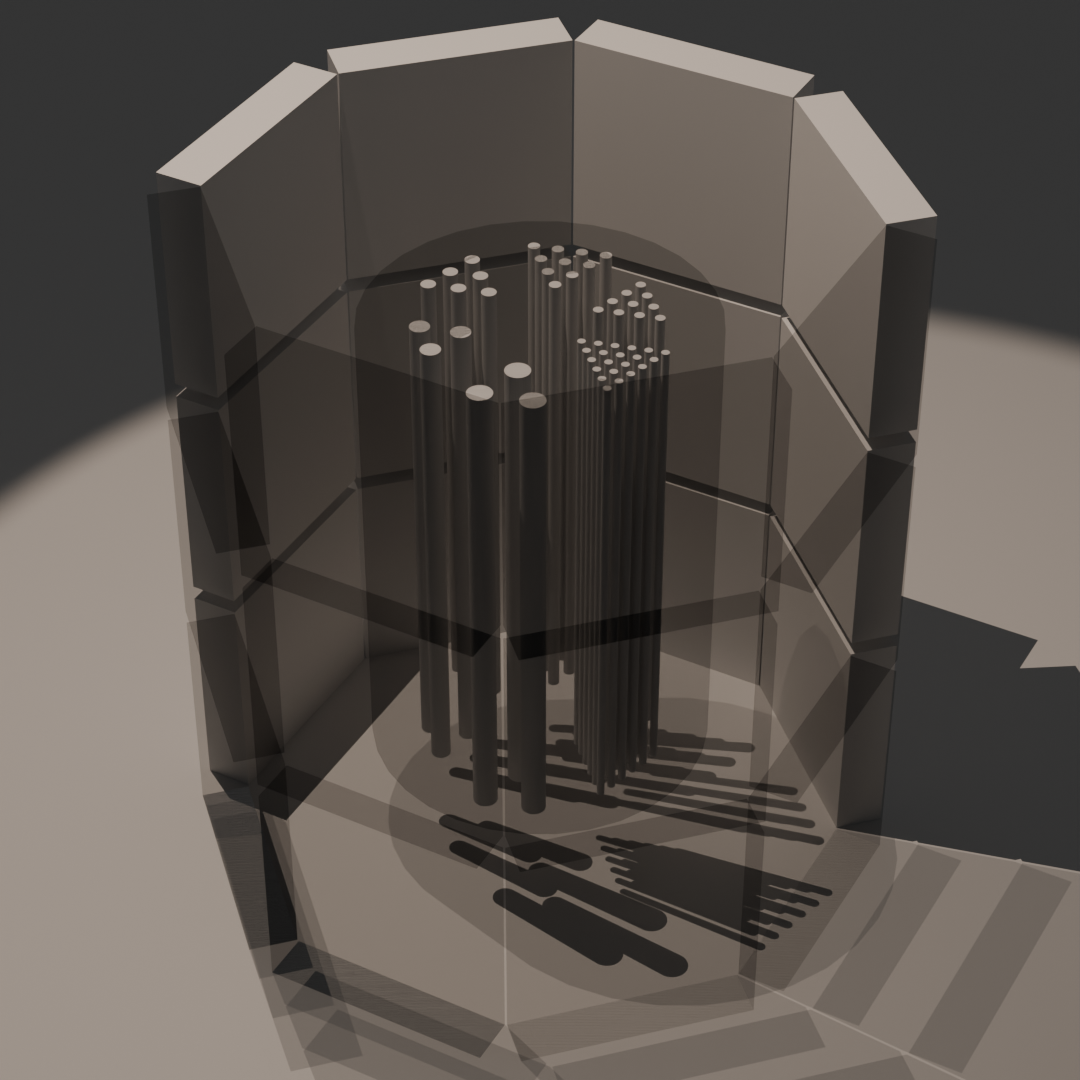
\includegraphics[height=4.5cm,keepaspectratio]{geometria_completa2.png}
            \vskip0.1cm
            {\scriptsize\color{mcmBlack!65} Figura 7. Modelado geométrico tridimensional del escáner Bruker PET/CT Si78 y el fantoma Derenzo en Blender.\par}
        \end{column}
    \end{columns}
    % NOTA DEL PONENTE: Modelamos con precisión submilimétrica los componentes clave. El Bruker Si78 se modeló como una geometría octogonal de tres anillos con cristales centelleadores de LYSO. El fantoma Derenzo digital replica el fantoma experimental con sus 6 sectores de varillas. Esta geometría se definió de forma visual y se exportó a cuádricas analíticas.
\end{frame}

% --- Diapositiva 8b: Métricas de Calidad de Imagen ---
\begin{frame}{Métricas de Calidad de Imagen}
    \begin{columns}[c]
        \begin{column}{0.52\textwidth}
            \colorbox{mcmPrimaryMuted}{\strut\textcolor{mcmPrimary}{\bfseries\scriptsize CONTRASTE}}
            \enskip \textbf{Coeficiente de Recuperación}
            \[ \text{CRC} = \frac{\textcolor{mcmPrimary}{\mu_{\text{hot}}}}{\mu_{\text{bkg}}} - 1 \]

            \vspace{0.4cm}

            \colorbox{mcmExampleBg}{\strut\textcolor{mcmExample}{\bfseries\scriptsize RUIDO}}
            \enskip \textbf{Relación Señal-Ruido}
            \[ \text{SNR} = \frac{\mu_{\text{bkg}}}{\textcolor{mcmExample}{\sigma_{\text{bkg}}}} \]
        \end{column}
        \begin{column}{0.44\textwidth}
            \centering
            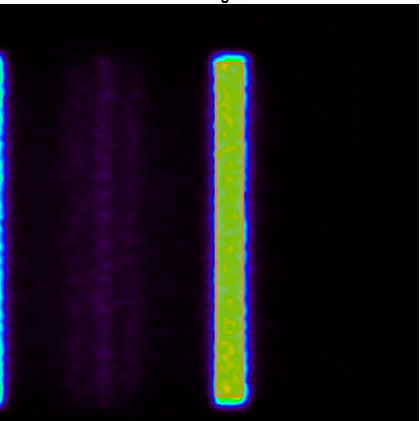
\includegraphics[height=4cm,keepaspectratio]{roi_amide.png}
            \vskip0.1cm
            {\scriptsize\color{mcmBlack!65} Figura 8. ROIs de varillas y fondo en AMIDE.\par}
        \end{column}
    \end{columns}
    \vspace{0.4cm}
    \centering
    {\scriptsize\color{mcmBlack!60}
        \boldmath\textcolor{mcmPrimary}{$\mu_{\text{hot}}$}\unboldmath: Media en varillas (Señal) \quad \textbullet \quad
        $\mu_{\text{bkg}}$, \boldmath\textcolor{mcmExample}{$\sigma_{\text{bkg}}$}\unboldmath: Media y Desviación Estándar en el fondo (Ruido)
    }
    % NOTA DEL PONENTE: Para evaluar la calidad de las imágenes reconstruidas de forma cuantitativa, utilizamos dos métricas principales: el Coeficiente de Recuperación de Contraste (CRC) y la Relación Señal-Ruido (SNR). El CRC compara la actividad media medida en las varillas calientes con la del fondo, restándole uno. El SNR mide el nivel de ruido en una región de fondo homogénea dividiendo su media por la desviación estándar. Como apoyo visual, a la derecha se muestran las Regiones de Interés (ROIs) cilíndricas que dibujamos sobre el fantoma Derenzo en el software AMIDE para realizar estas medidas de forma reproducible.
\end{frame}

% --- Diapositiva 9 ---
\begin{frame}{Simulación Monte Carlo: Definiciones Clave}
    \begin{columns}[T]
        \begin{column}{0.54\textwidth}
            \begin{block}{Conceptos Fundamentales}
                \begin{itemize}
                    \item \textbf{History (Historia):}\\Unidad de simulación (partícula primaria + secundarias).
                          \vspace{0.3cm}
                    \item \textbf{Singles:}\\Registro de fotones individuales (tiempo, energía e ID).
                \end{itemize}
            \end{block}
        \end{column}
        \begin{column}{0.42\textwidth}
            \centering
            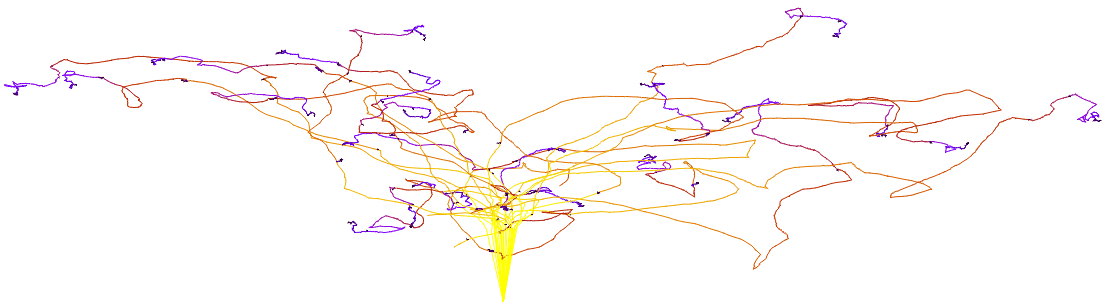
\includegraphics[width=\textwidth]{particle_track.png}
            \vskip0.1cm
            {\scriptsize\color{mcmBlack!65} Figura 9. Visualización del transporte de trazas de electrones en agua simulados en \penred.\par}
            \vskip0.2cm
            \begin{exampleblock}{Ficheros}
                \begin{itemize}
                    \item Ejecutable (\penred)
                    \item Configuración
                    \item Geometría
                \end{itemize}
            \end{exampleblock}
        \end{column}
    \end{columns}
    \vspace{0.2cm}
    % NOTA DEL PONENTE: Para entender la simulación computacional de este proyecto, es vital tener claros tres conceptos de Monte Carlo. Primero, la "Historia", que es el seguimiento completo desde que la fuente emite un decaimiento hasta que todas las partículas resultantes se detienen. Segundo, los "Tallies", que son nuestros detectores virtuales que guardan la información. Y tercero, los "Singles", el tally específico que registra cada evento de deposición de energía de forma cruda antes de formar coincidencias. Todo esto fue orquestado en penRed usando cuatro ficheros clave (ejecutable, configuración, geometría y materiales) que fueron enviados al supercomputador Quasar de la universidad, donde simulamos nada menos que 1500 millones de historias con alta precisión.
\end{frame}

% --- Diapositiva 10 ---
\begin{frame}{Diseño Experimental: Fases 1 y 2}
    \begin{itemize}
        \item \textbf{Estadística simulada:} $2\cdot 10^8$ historias (\SI{27.77}{\kilo\becquerel} en 2\,h).
    \end{itemize}
    \vspace{-0.1cm}
    \begin{block}{Fase 1: Validación Ideal (Ground Truth)}
        \begin{itemize}
            \item \textbf{Configuración:} Vacío (\texttt{void}) y detectores perfectos.
                  \begin{itemize}
                      \item \scriptsize Se fuerza la aniquilación \textit{in situ} del $\beta^+$ (elimina el rango del positrón en vacío).
                  \end{itemize}
            \item \textbf{Post-procesado:} Modo \ingles{Same History} ($0\%$ aleatorios).
            \item \textbf{Objetivo:} Referencia libre de atenuación, scatter y aleatorios.
        \end{itemize}
    \end{block}
    \begin{block}{Fase 2: Scatter y Atenuación}
        \begin{itemize}
            \item \textbf{Configuración:} Fantoma de agua, detectores LYSO realistas.
            \item \textbf{Post-procesado:} Modo \ingles{Same History} ($0\%$ aleatorios).
            \item \textbf{Objetivo:} Aislar el impacto Compton y atenuación en agua/cristal.
        \end{itemize}
    \end{block}
    % NOTA DEL PONENTE: La metodología propone un enfoque incremental. En la Fase 1 establecemos el Ground Truth definiendo todo como vacío. Como detalle técnico, en el vacío el positrón no tendría materia con la que aniquilarse, por lo que forzamos su aniquilación in situ en el simulador. Esto genera los fotones de 511 keV y elimina por completo el emborronamiento por el rango del positrón, dándonos una referencia perfecta. En la Fase 2 añadimos agua y detectores realistas para aislar el scatter Compton y la atenuación.
\end{frame}

% --- Diapositiva 11 ---
\begin{frame}{Diseño Experimental: Fases 3, 4 y 5}
    \begin{block}{Fases Metodológicas Finales}
        \begin{itemize}\setlength{\itemsep}{0.8em}
            \item \textbf{Fase 3 (Línea Base):} Mismos datos de Fase 2 (\SI{27.77}{\kilo\becquerel}). Se usa el modo \ingles{Take Closest} (CW: $5$\,ns y EW: $30\%$) para añadir coincidencias aleatorias.
            \item \textbf{Fase 4 (Optimización):} Barrido paramétrico (EW: $20\%$, $15\%$, $10\%$ y CW: $4$, $3$\,ns). \alert{Estadística ampliada:} $1.5 \cdot 10^9$ historias (\SI{208.3}{\kilo\becquerel}).
            \item \textbf{Fase 5 (mPET):} Adquisición dual simultánea con \fdiezocho y \yochoseis, clasificando triples para la separación de trazadores.
        \end{itemize}
    \end{block}
    % NOTA DEL PONENTE: En la Fase 4 realizamos un estudio paramétrico barriendo la Ventana de Energía (EW) y la Ventana de Coincidencia (CW) para buscar el punto óptimo de funcionamiento. En la Fase 5, validamos el multiplexado (mPET) simulando un fantoma dual cargado con F-18 y Y-86 de forma simultánea.
\end{frame}

% --- Diapositiva 12 ---
\begin{frame}{Desarrollo en C++: Post-procesado}
    \begin{columns}[T]
        \begin{column}{0.54\textwidth}
            \begin{block}{El Software \texttt{createCoincidences}}
                \begin{itemize}
                    \item Añade efectos del detector no simulables nativamente en \penred.
                    \item \textbf{Modelado de Hardware (Blurring):}
                          \begin{itemize}
                              \item \textbf{Energético:} 14\% FWHM a \SI{511}{\kilo\electronvolt}.
                              \item \textbf{Espacial:} Resolución intrínseca de 0.08\,cm.
                          \end{itemize}
                    \item \textbf{Lógica:} Buffer deslizante y aplicación de ventanas (CW y EW).
                \end{itemize}
            \end{block}
        \end{column}
        \begin{column}{0.42\textwidth}
            \centering
            
\includegraphics[height=4.2cm,keepaspectratio]{materiales_colores.png}
            \vskip0.1cm
            {\scriptsize\color{mcmBlack!65} Figura 10. Definición espacial y geométrica de materiales y componentes del escáner.\par}
        \end{column}
    \end{columns}
    % NOTA DEL PONENTE: Uno de los pilares del proyecto es el software propio createCoincidences desarrollado en C++. penRed simula física ideal, por lo que es necesario nuestro código para modelar la electrónica del escáner real. Este software lee los "singles", aplica el desenfoque o "blurring" gaussiano (resolución espacial, energética y temporal), e implementa la lógica de emparejamiento. Es aquí exactamente donde definimos las ventanas de energía (EW) y de coincidencia (CW) con las que el buffer deslizante filtra y extrae las coincidencias.
\end{frame}

% --- Diapositiva 13 ---
\begin{frame}[fragile]{Desarrollo en C++: Lógica de Triples}
    \begin{columns}[T]
        \begin{column}{0.48\textwidth}
            \begin{block}{Detección de Triples}
                \begin{itemize}
                    \item \textbf{PET Doble:} Coincidencia temporal estándar.
                    \item \textbf{Prompt Gamma:} Busca un tercer single en el rango $650 - 2000$\,keV.
                          \begin{itemize}
                              \item \scriptsize Umbral alto: minimiza la aceptación de gammas dispersados (\textit{scatter}).
                          \end{itemize}
                    \item \textbf{Salida Dual LM:}
                          \begin{itemize}
                              \item \texttt{data\_AB.lm}: Dobles (mixtas).
                              \item \texttt{data\_B\_prime.lm}: Triples de \yochoseis.
                          \end{itemize}
                \end{itemize}
            \end{block}
        \end{column}
        \begin{column}{0.48\textwidth}
            \begin{block}{Código C++ de Clasificación}
                \begin{lstlisting}[language=C++, basicstyle=\ttfamily\tiny, keywordstyle=\color{blue}, commentstyle=\color{green!60!black}, breaklines=true]
// Filter standard PET singles
if (nextSingles[i].e > emax) continue;
iCoincidence = i; iPair = localPair;

// Scan for Prompt Gamma (Triple)
for (size_t k = 0; k < nextSingles.size(); ++k) {
  if (k == 0 || k == i) continue;
  if (nextSingles[k].e >= promptGammaThreshold) {
    isTriple = true; // Event classified
    break;
  }
}
\end{lstlisting}
            \end{block}
        \end{column}
    \end{columns}
    \vspace{0.1cm}
    \hfill {\tiny\color{mcmBlack!40} [Andreyev et al., 2011]}
    % NOTA DEL PONENTE: Aquí muestro la lógica del algoritmo de multiplexado. Buscamos la pareja convencional de 511 keV. Si en su ventana temporal detectamos un tercer fotón con energía superior a 650 keV, lo clasificamos como triple. Este umbral alto es crítico: minimiza la inclusión de prompt gammas que han sufrido dispersión Compton, las cuales degradarían la resolución espacial. Finalmente, guardamos dos datasets independientes en modo lista.
\end{frame}

% =====================================================================
% SECCIÓN 3: RESULTADOS Y DISCUSIÓN
% =====================================================================
\section{Resultados y Discusión}

% --- Diapositiva 14 ---
\begin{frame}{Validación del Espectro del Itrio-86}
    \begin{columns}[T]
        \begin{column}{0.38\textwidth}
            \begin{block}{Verificación Física}
                \begin{itemize}
                    \item Espectro de singles extraído en vacío.
                    \item Excelente correspondencia entre fotopicos simulados y datos teóricos NuDat 3.
                \end{itemize}
            \end{block}
            \vskip-0.2cm
            \begin{table}
                \centering
                \scriptsize
                \begin{tabular}{l c c}
                    \toprule
                    \textbf{Origen}   & \textbf{Teórico (keV)} & \textbf{Simulado (keV)} \\
                    \midrule
                    Aniquilación      & 511.0                  & 511                     \\
                    Prompt $\gamma_1$ & 627.7                  & $\sim 628$              \\
                    Prompt $\gamma_2$ & 1076.6                 & $\sim 1077$             \\
                    Prompt $\gamma_3$ & 1153.1                 & $\sim 1153$             \\
                    \bottomrule
                \end{tabular}
            \end{table}
        \end{column}
        \begin{column}{0.58\textwidth}
            \centering
            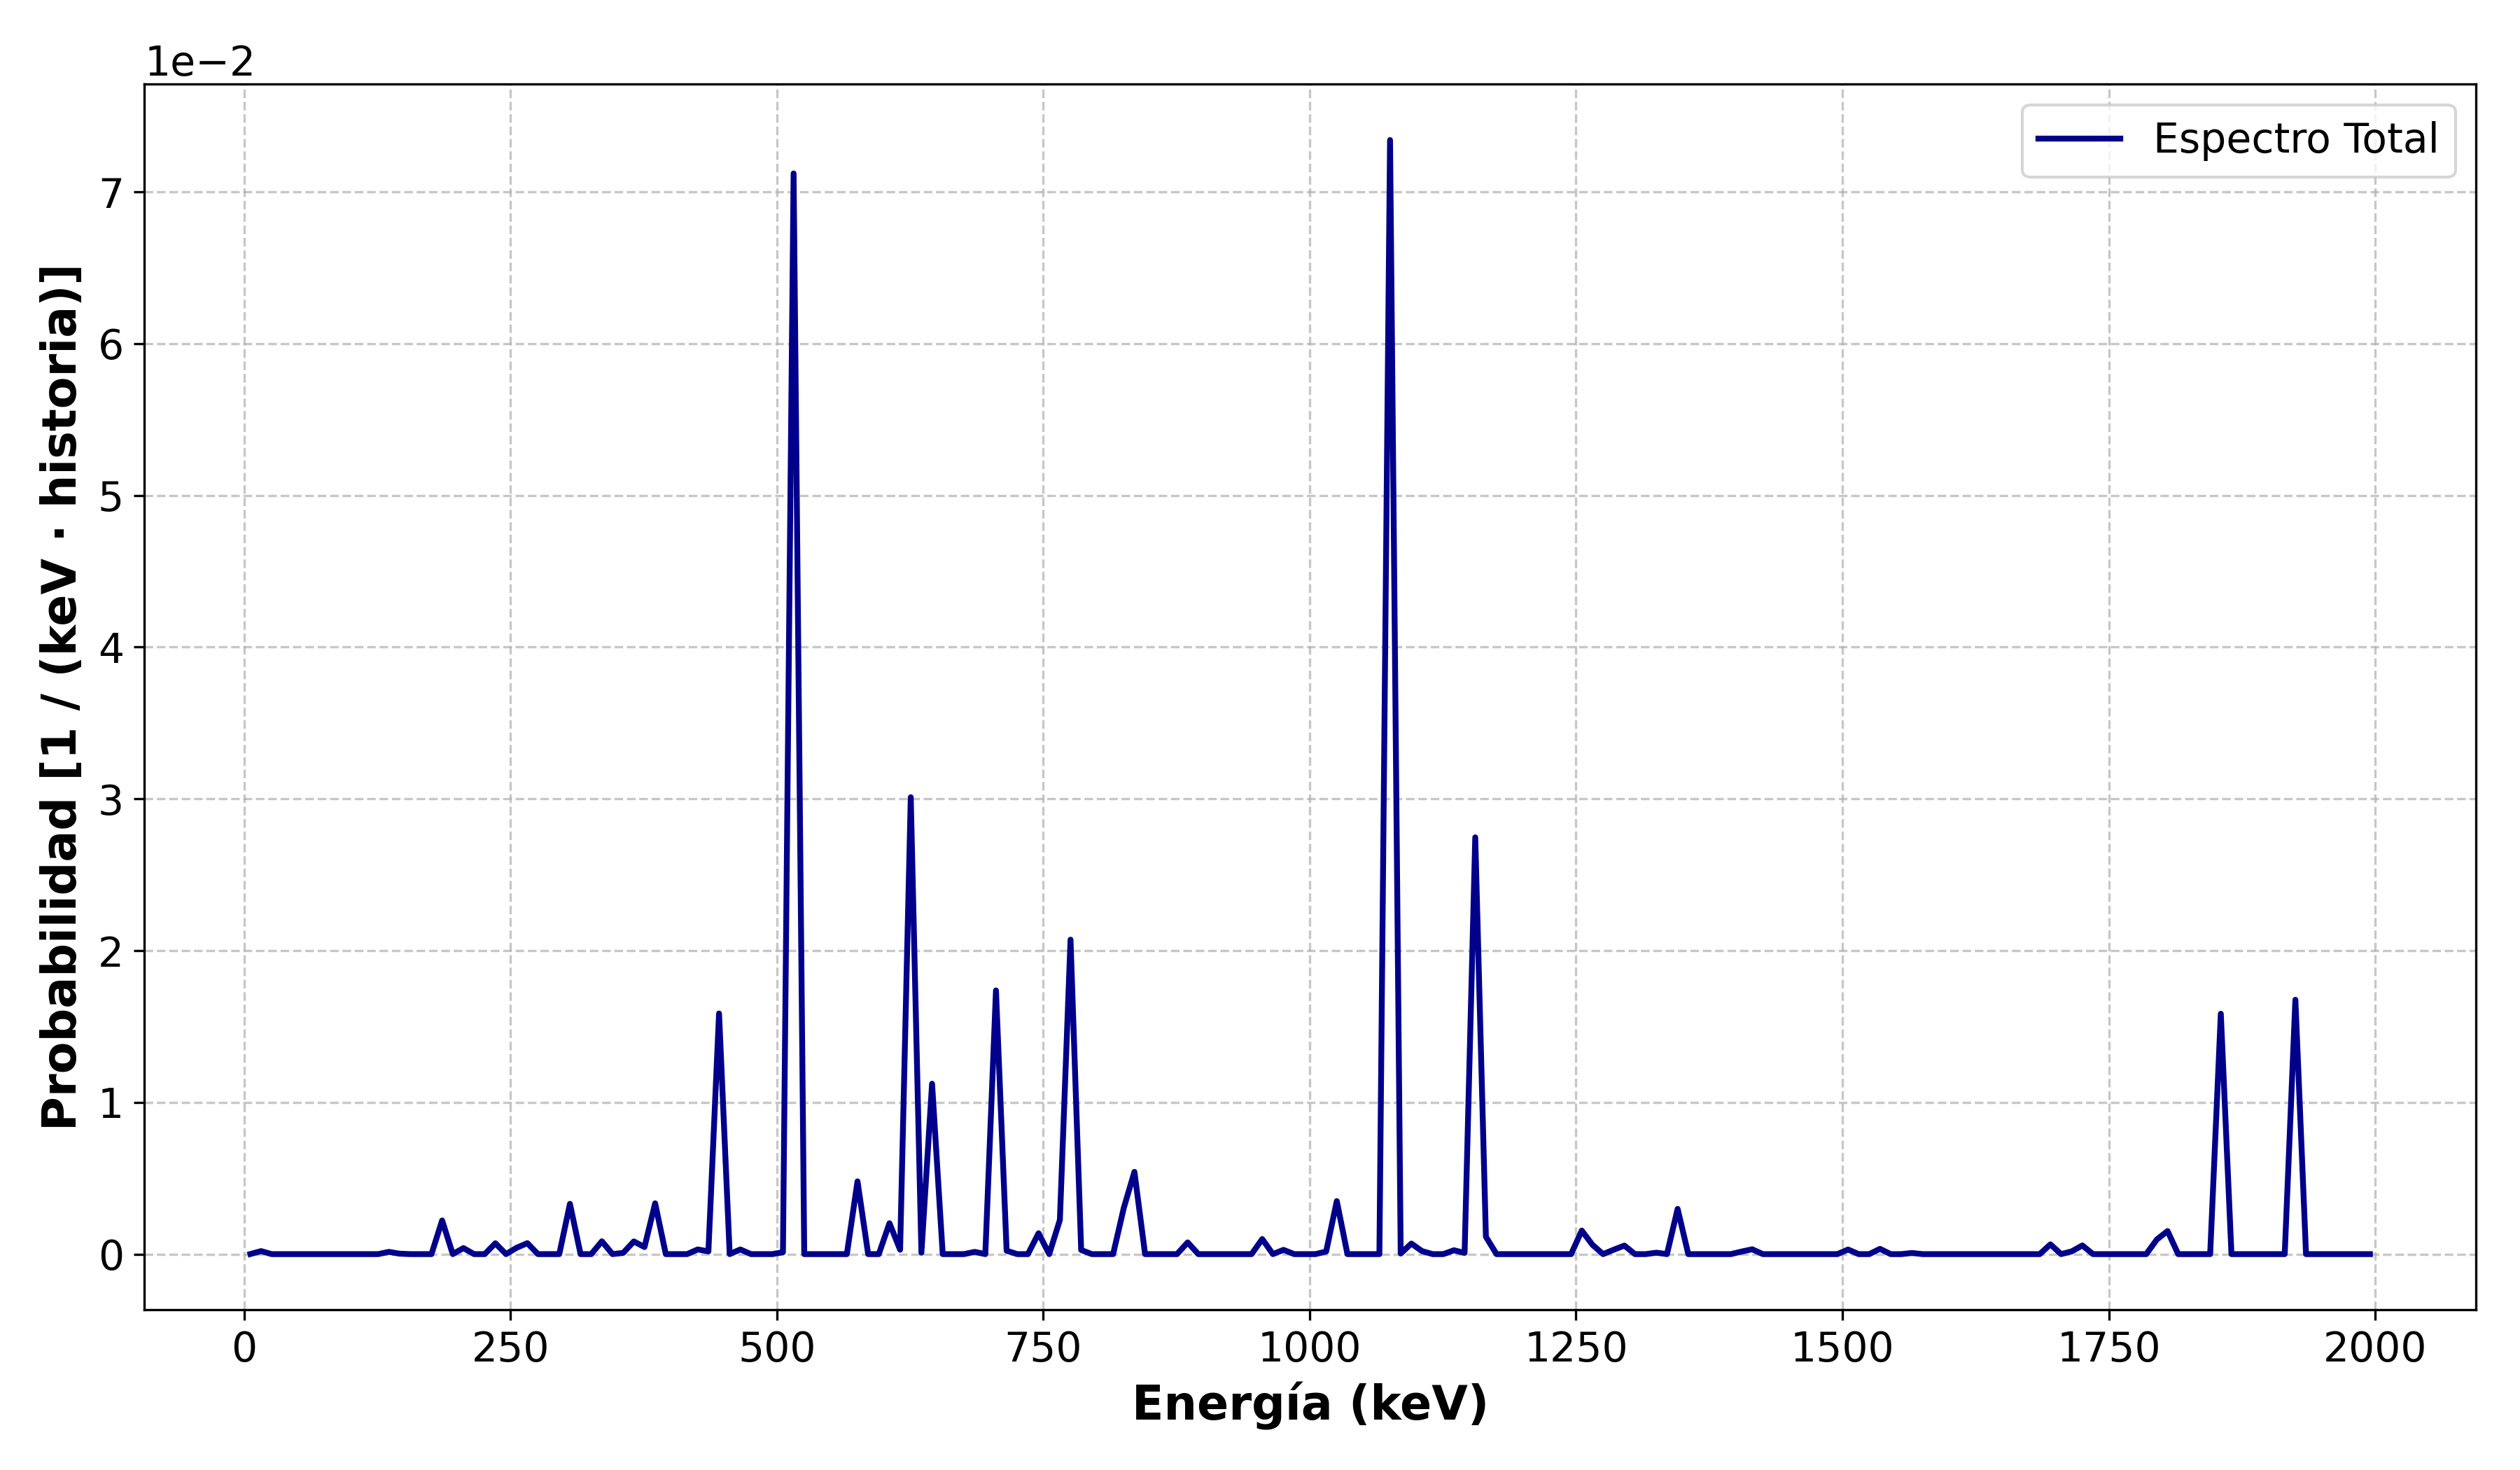
\includegraphics[width=\textwidth]{espectro_energia_kev_y_kev.png}
            \vskip0.1cm
            {\scriptsize\color{mcmBlack!65} Figura 11. Espectro simulado de depósito de energía de singles de \yochoseis en vacío.\par}
        \end{column}
    \end{columns}
    % NOTA DEL PONENTE: Entramos en la sección de Resultados. El primer paso fue validar la física de desintegración nuclear. Al simular en vacío, el histograma de singles muestra de forma discreta los fotopicos teóricos. Identificamos perfectamente el de 511 keV de aniquilación y las líneas de prompt gammas a 628, 1077 y 1153 keV, con energías idénticas a los datos oficiales de NuDat 3. Esto confirma la validez de nuestro modelo físico.
\end{frame}

% --- Diapositiva 15 ---
\begin{frame}{Simulación Ideal (Fase 1: Ground Truth)}
    \begin{columns}[T]
        \begin{column}{0.48\textwidth}
            \begin{block}{Resultados de la Fase 1}
                \begin{itemize}
                    \item Ausencia total de ruido y dispersión Compton.
                    \item Varillas finas (\SI{0.8}{\milli\meter}) totalmente resueltas.
                    \item El modo \ingles{Same History} elimina todo el fondo espurio.
                    \item \textbf{CRC de Referencia:} \alert{185.27}.
                \end{itemize}
            \end{block}
        \end{column}
        \begin{column}{0.48\textwidth}
            \centering
            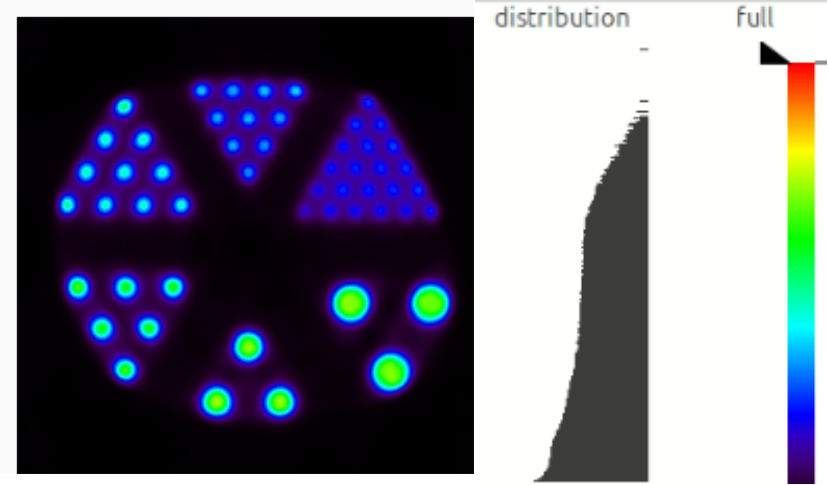
\includegraphics[height=4cm,keepaspectratio]{IMG_IDEAL_Y86.png}
            \vskip0.1cm
            {\scriptsize\color{mcmBlack!65} Figura 12. Reconstrucción tomográfica ideal MLEM (Fase 1: Ground Truth).\par}
        \end{column}
    \end{columns}
    % NOTA DEL PONENTE: Reconstruyendo en condiciones ideales de la Fase 1, obtenemos una imagen de referencia perfecta de nuestro fantoma Derenzo. Al no haber medio dispersor y aplicar el Same History, el contraste es óptimo con un CRC de 185.27. Las varillas más pequeñas de 0.8 mm están perfectamente resueltas. Este es el techo teórico de calidad de nuestro sistema.
\end{frame}

% --- Diapositiva 16 ---
\begin{frame}{Caracterización de la Degradación (Fase 2)}
    \begin{columns}[T]
        \begin{column}{0.48\textwidth}
            \begin{block}{Impacto de Scatter y Atenuación}
                \begin{itemize}
                    \item El scatter Compton en agua y LYSO genera halos difusos.
                    \item El CRC cae de \textbf{185.27} a \alert{11.57} (\alert{pérdida de contraste del 93.7\%}).
                    \item El \textbf{SNR} resultante es de \textbf{3.13}.
                    \item \textbf{Causa:} Dispersión de prompt gammas de alta energía.
                \end{itemize}
            \end{block}
        \end{column}
        \begin{column}{0.48\textwidth}
            \centering
            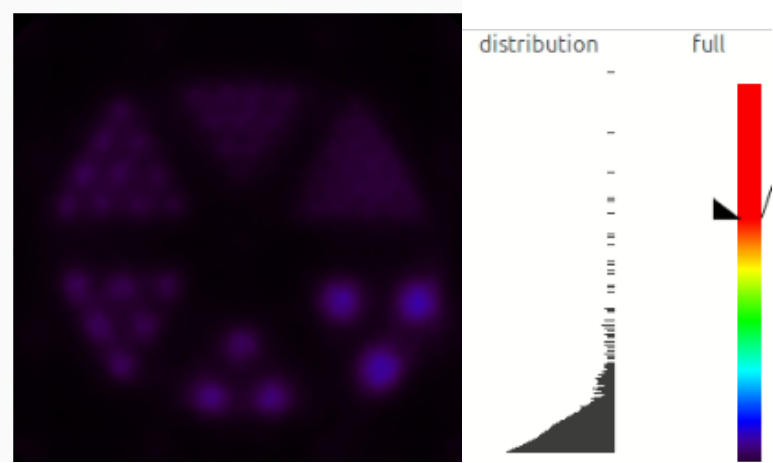
\includegraphics[height=4cm,keepaspectratio]{IMG_SCATTER_Y86.png}
            \vskip0.1cm
            {\scriptsize\color{mcmBlack!65} Figura 13. Imagen reconstruida de \yochoseis bajo el efecto de scatter y atenuación en agua (Fase 2).\par}
        \end{column}
    \end{columns}
    % NOTA DEL PONENTE: Al introducir agua en la Fase 2, el contraste colapsa dramáticamente cayendo a 11.57. Es una pérdida de contraste del 93.7%. En la imagen de la derecha apreciamos cómo las varillas pequeñas se emborronan debido a los halos Compton generados por los fotones dispersados en el agua, los cuales contaminan la región fría.
\end{frame}

% --- Diapositiva 17 ---
\begin{frame}{Caracterización de la Degradación (Fase 3)}
    \begin{columns}[T]
        \begin{column}{0.48\textwidth}
            \begin{block}{Impacto de Coincidencias Aleatorias}
                \begin{itemize}
                    \item La lógica realista de emparejamiento de coincidencia ({Take Closest}) añade aleatorios.
                    \item El CRC es estable (\textbf{11.73}), pero el \textbf{SNR cae un 12.5\%} a \alert{2.74}.
                    \item \textbf{Conclusión física:} El scatter Compton de prompt gammas daña el contraste (CRC), y los aleatorios añaden ruido (SNR).
                \end{itemize}
            \end{block}
        \end{column}
        \begin{column}{0.48\textwidth}
            \centering
            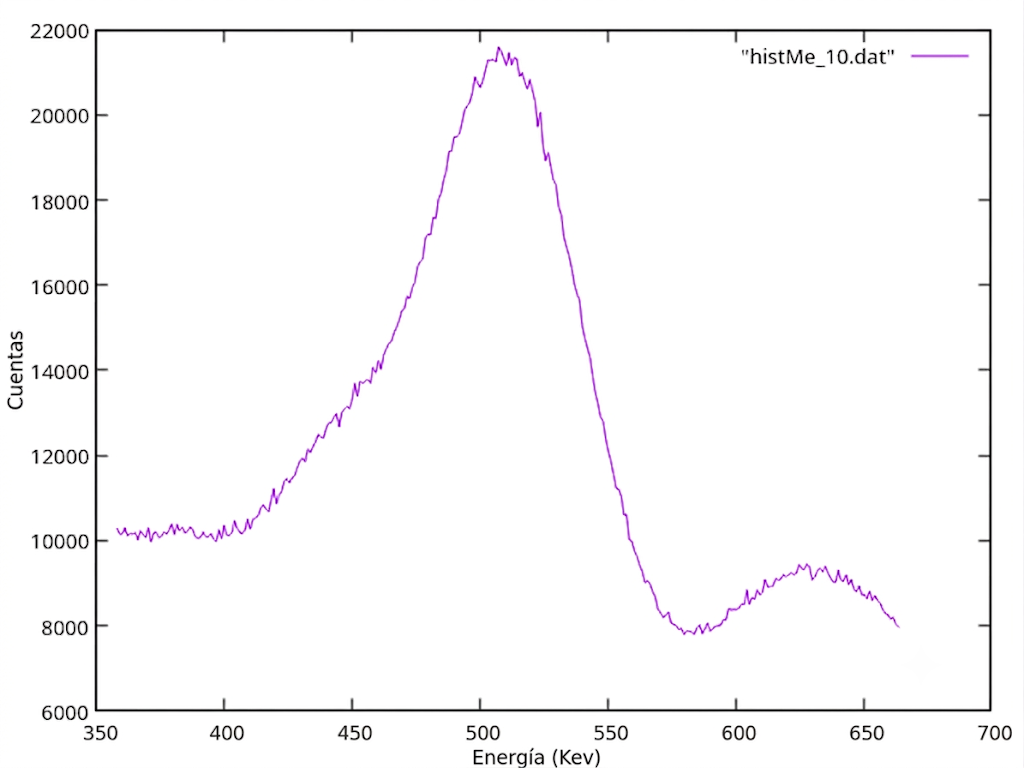
\includegraphics[height=4.8cm,keepaspectratio]{espectro_det10_SIM_RANDOMS.png}
            \vskip0.1cm
            {\scriptsize\color{mcmBlack!65} Figura 14. Espectro realista de energía final registrado en los detectores (Fase 3).\par}
        \end{column}
    \end{columns}
    % NOTA DEL PONENTE: Al pasar a la simulación realista final de la Fase 3, donde no hay filtros de historia, introducimos las coincidencias aleatorias. El CRC se mantiene muy similar a la Fase 2, pero el SNR baja un 12.5% hasta 2.74. La conclusión física es que el scatter Compton de los prompt gammas dicta la pérdida de contraste (CRC), y las coincidencias aleatorias son las que añaden ruido estadístico general.
\end{frame}

% --- Diapositiva 18 ---
\begin{frame}{Comparativa Crítica: \yochoseis vs \fdiezocho}
    \begin{columns}[T]
        \begin{column}{0.54\textwidth}
            \begin{block}{\fdiezocho (Limpio) vs. \yochoseis (Sucio)}
                \begin{itemize}
                    \item Comparación bajo idéntica geometría y electrónica.
                    \item El \yochoseis presenta contraste \alert{2.6 veces inferior} y \alert{29\% menos de SNR} debido al fondo de prompt gammas.
                \end{itemize}
            \end{block}
        \end{column}
        \begin{column}{0.42\textwidth}
            \centering
            \begin{table}
                \centering
                \scriptsize
                \begin{tabular}{l c c}
                    \toprule
                    \textbf{Isótopo}    & \textbf{CRC} & \textbf{SNR} \\
                    \midrule
                    \fdiezocho (Limpio) & 31.09        & 3.86         \\
                    \yochoseis (Sucio)  & 11.73        & 2.74         \\
                    \bottomrule
                \end{tabular}
            \end{table}
        \end{column}
    \end{columns}
    \vskip0.05cm
    \centering
    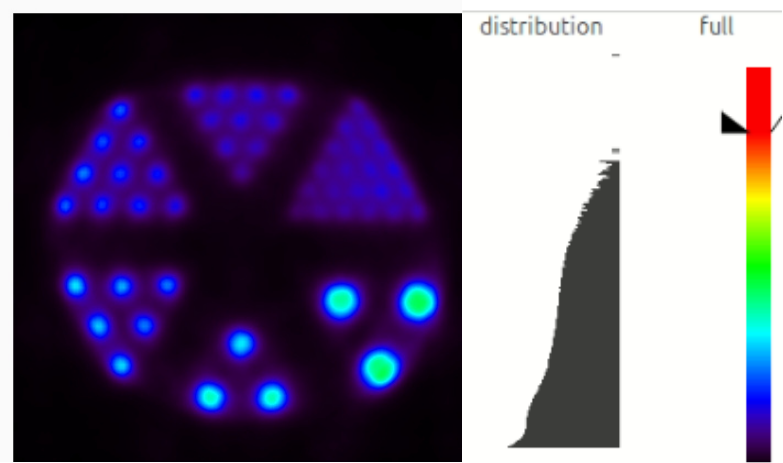
\includegraphics[width=0.29\textwidth,height=2.7cm,keepaspectratio]{IMG_CLOSEST_TIME-F18.png}
    \hspace{0.3cm}
    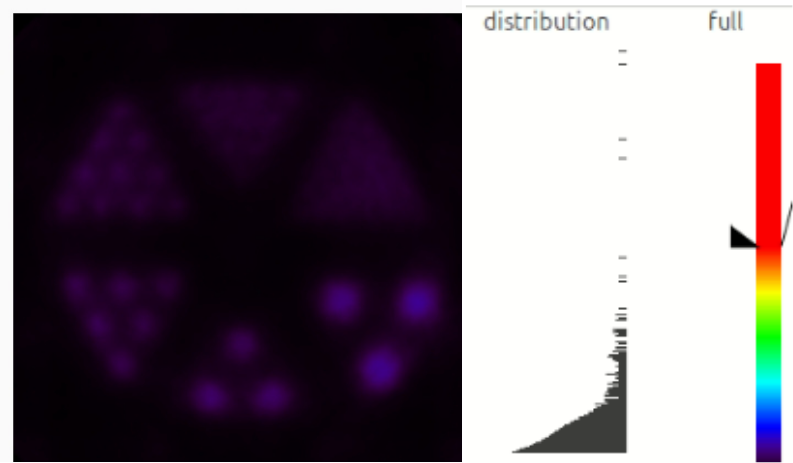
\includegraphics[width=0.29\textwidth,height=2.7cm,keepaspectratio]{IMG_CLOSEST_TIME-Y86.png}
    \vskip0.05cm
    {\scriptsize\color{mcmBlack!65} Figura 15. Comparativa de reconstrucciones en condiciones reales: \fdiezocho (izquierda) e \yochoseis (derecha) bajo idénticos parámetros de adquisición.\par}
    % NOTA DEL PONENTE: Para aislar el efecto de los prompt gammas, simulamos el Fluor-18, emisor beta+ puro, bajo los mismos parámetros. El contraste del F-18 es de 31.09 frente al 11.73 del Y-86. El Y-86 sufre una caída de contraste de 2.6 veces y un ruido muy superior debido puramente a los prompt gammas. Esto justifica metodológicamente la necesidad de optimizar las ventanas del detector.
\end{frame}

% --- Diapositiva 19 ---
\begin{frame}{Optimización: Ventana de Energía (EW)}
    \begin{block}{Reducción de la Ventana EW}
        \begin{itemize}
            \item Evaluada con ventana temporal fija (CW = 4\,ns).
            \item Reducir EW al $10\%$ ($460$-$562$\,keV) logra un \alert{aumento del 79\% en el contraste} (CRC sube de \textbf{10.73} a \textbf{19.17}).
            \item El SNR disminuye levemente (de \textbf{7.53} a \textbf{6.64}) por la pérdida de sensibilidad.
        \end{itemize}
    \end{block}
    \centering
    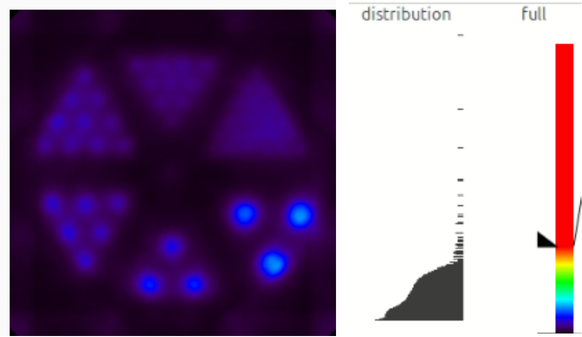
\includegraphics[width=0.29\textwidth,height=2.5cm,keepaspectratio]{IMG_OPT_EW1_CW1.png}
    \hspace{0.1cm}
    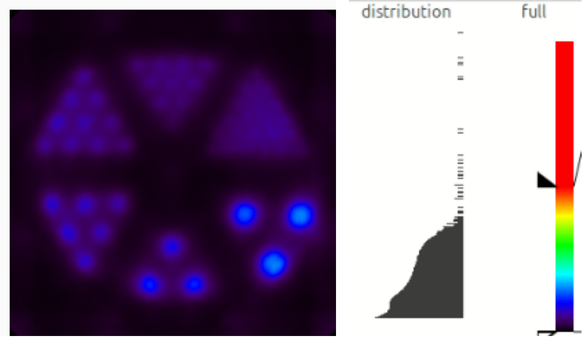
\includegraphics[width=0.29\textwidth,height=2.5cm,keepaspectratio]{IMG_OPT_EW2_CW1.png}
    \hspace{0.1cm}
    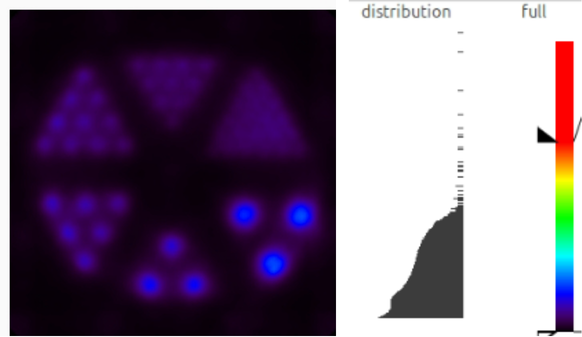
\includegraphics[width=0.29\textwidth,height=2.5cm,keepaspectratio]{IMG_OPT_EW3_CW1.png}
    \vskip0.05cm
    {\scriptsize\color{mcmBlack!65} Figura 16. Efecto visual de la reducción de la ventana de energía (20\% izquierda, 15\% centro, 10\% derecha).\par}
    % NOTA DEL PONENTE: Evaluamos la optimización estrechando la ventana de energía (EW) para bloquear el scatter Compton y prompt gammas. Al bajar la ventana del 30% al 10%, el CRC mejora un 79%, duplicando el contraste y pasando de 10.73 a 19.17. La penalización de ruido es mínima, con el SNR variando ligeramente de 7.53 a 6.64. Visualmente, se recupera el contraste en las varillas de 1.2 mm.
\end{frame}

% --- Diapositiva 20 ---
\begin{frame}{Optimización: Ventana CW y Trade-off}
    \begin{columns}[T]
        \begin{column}{0.50\textwidth}
            \begin{block}{Efecto de la Ventana Temporal}
                \begin{itemize}
                    \item Reducir CW a 3\,ns disminuye aleatorios y mejora SNR en 1-5\%, sin impacto en el contraste.
                    \item EW es el parámetro físico dominante.
                \end{itemize}
            \end{block}
            \begin{exampleblock}{Punto de Trabajo Óptimo}
                \begin{itemize}
                    \item La combinación \alert{EW 10\% / CW 4\,ns} da el contraste máximo (CRC = 19.17) y ruido controlado (SNR = 6.64).
                \end{itemize}
            \end{exampleblock}
        \end{column}
        \begin{column}{0.46\textwidth}
            \centering
            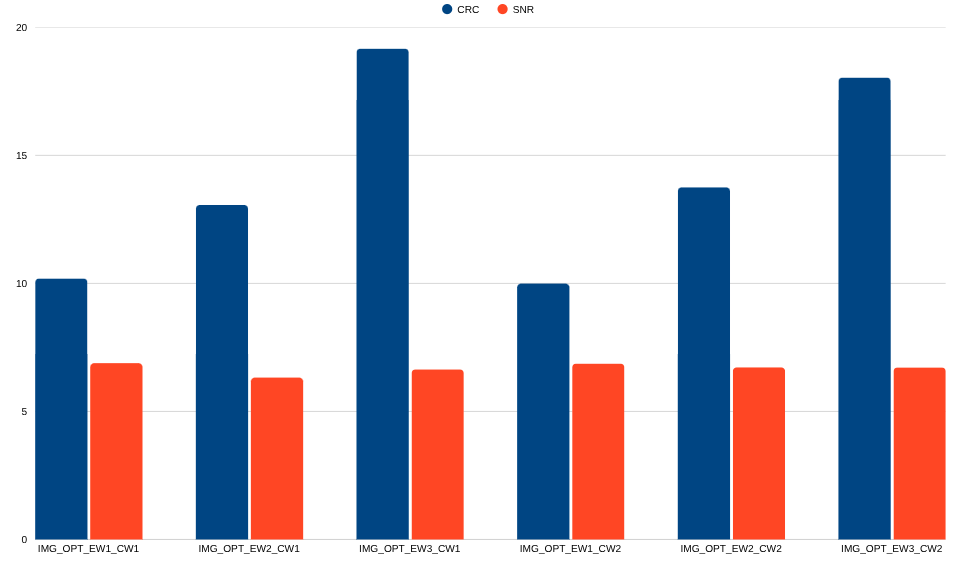
\includegraphics[height=4.8cm,keepaspectratio]{tradeoff.png}
            \vskip0.1cm
            {\scriptsize\color{mcmBlack!65} Figura 17. Relación de compromiso entre contraste (CRC) y ruido (SNR) en función de la ventana EW.\par}
        \end{column}
    \end{columns}
    % NOTA DEL PONENTE: Analizamos el efecto de la ventana de coincidencia temporal (CW). Acortar de 4 a 3 ns solo genera una mejora marginal en el ruido (del 1-5%) y no influye en el contraste. Por tanto, confirmamos que la ventana de energía es la variable dominante. El punto óptimo de funcionamiento que proponemos es EW 10% / CW 4ns, maximizando la detectabilidad de structures pequeñas.
\end{frame}

% --- Diapositiva 22 ---
\begin{frame}{Prueba de Concepto mPET: Metodología}
    \begin{columns}[T]
        \begin{column}{0.54\textwidth}
            \begin{block}{Algoritmo de Sustracción Lineal}
                \begin{itemize}
                    \item \textbf{Adquisición:} Varilla izq. con \fdiezocho, varilla der. con \yochoseis.
                    \item \textbf{Clasificación:} Separa dobles mixtos ($I_{AB}$) y triples de \yochoseis ($I_{Y86}^T$).
                    \item \textbf{Estimación:} Contaminación en dobles: $I_{Y86}^D \approx 75.86 \cdot I_{Y86}^T$.
                    \item \textbf{Sustracción:} $I_{F18} = I_{AB} - 75.86 \cdot \text{smooth}(I_{Y86}^T)$.
                \end{itemize}
            \end{block}
        \end{column}
        \begin{column}{0.42\textwidth}
            \centering
            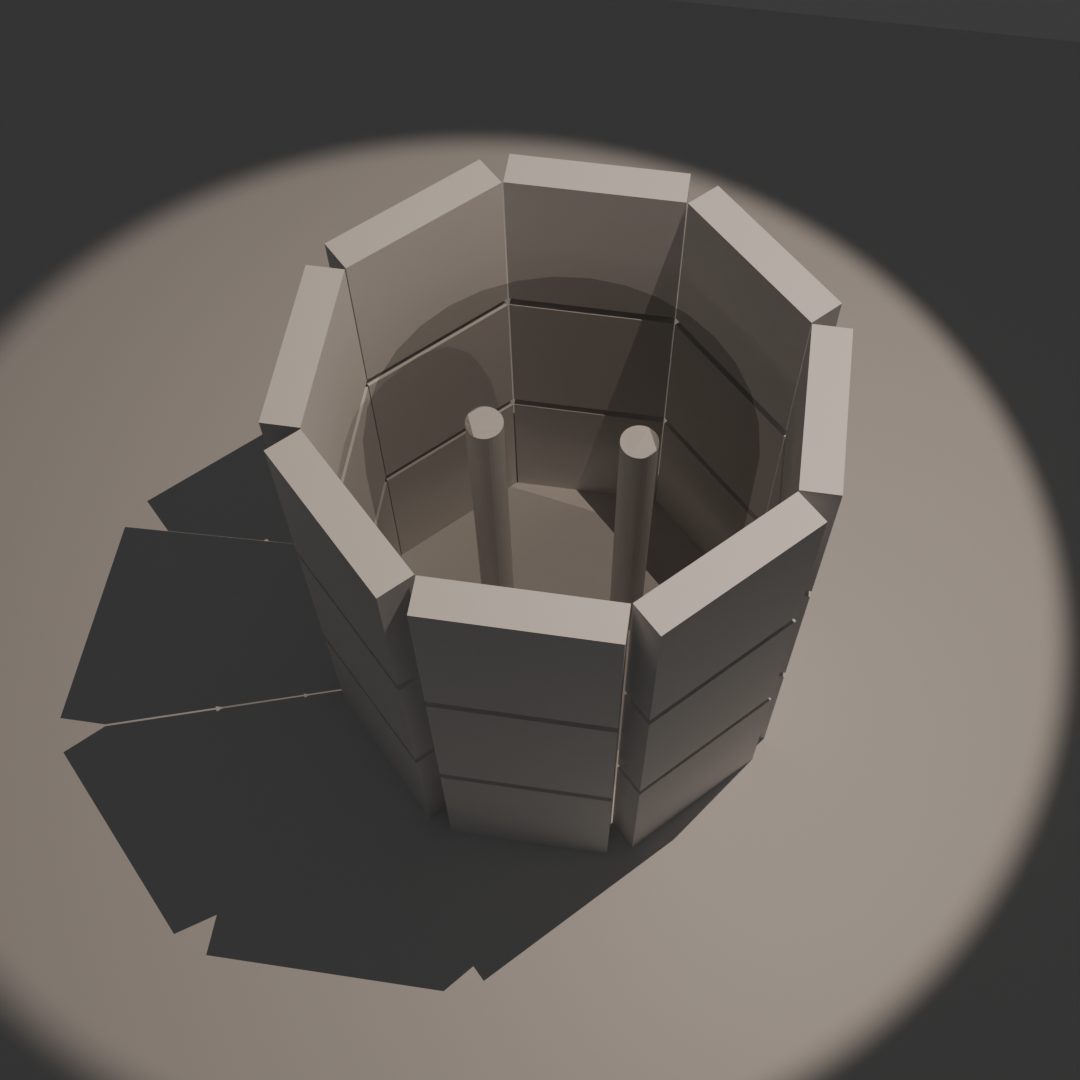
\includegraphics[height=4.2cm,keepaspectratio]{modelo_fantoma_mp.png}
            \vskip0.1cm
            {\scriptsize\color{mcmBlack!65} Figura 18. Geometría del fantoma cilindro dual simulado para la adquisición mPET simultánea.\par}
        \end{column}
    \end{columns}
    \vspace{0.2cm}
    \hfill {\tiny\color{mcmBlack!40} [Pratt et al., 2023]}
    % NOTA DEL PONENTE: Pasamos al objetivo estrella: el multiplexado mPET. Simulamos una varilla con F-18 y otra con Y-86. A partir de los datos binarios de singles, nuestro post-procesado genera el dataset mixto AB y el dataset puro de triples B'. En Python, aplicamos un factor empírico F = 75.86 para escalar los triples del Y-86 a su nivel de contaminación en dobles, y tras aplicar un filtro de suavizado gaussiano realizamos la sustracción.
\end{frame}

% --- Diapositiva 22 ---
\begin{frame}{Prueba de Concepto mPET: Resultados}
    \vspace{-0.2cm}
    \begin{center}
        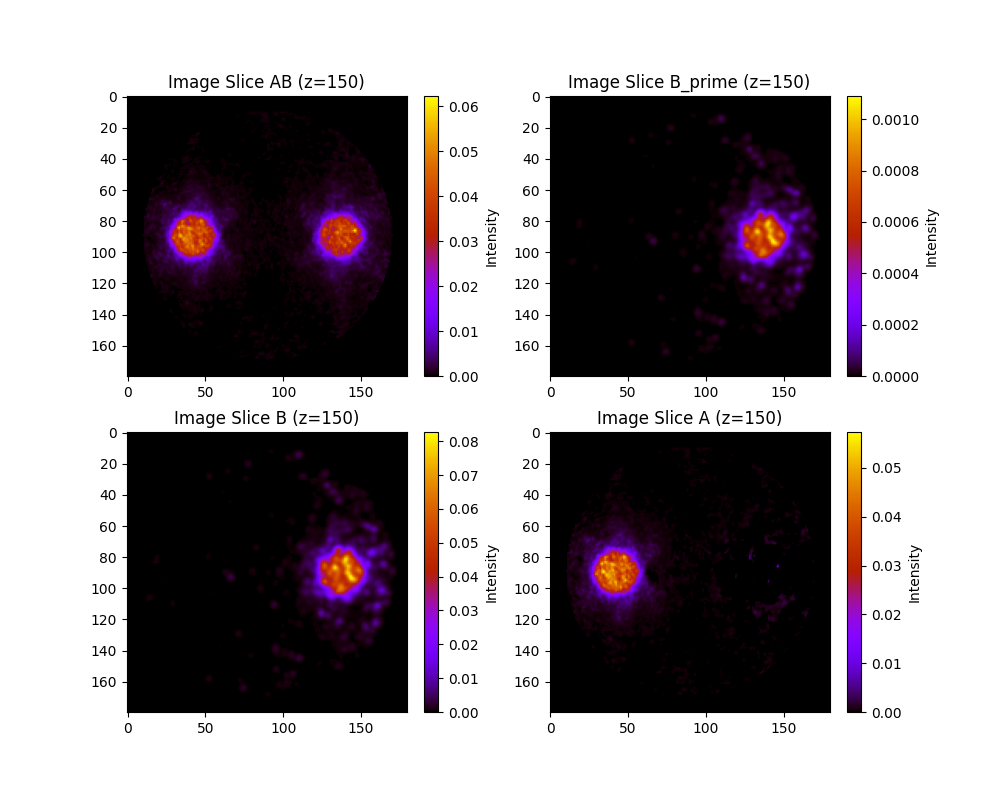
\includegraphics[height=6.4cm,keepaspectratio]{imagen_cuatro_subplots.png}
        \vskip0.1cm
        {\scriptsize\color{mcmBlack!65} Figura 19. Distribuciones de actividad en multiplexado: mixta (AB), Y-86 aislado con triples ($B'$) y F-18 puro recuperado ($A$).\par}
    \end{center}
    % NOTA DEL PONENTE: El resultado de la separación es excelente. En el panel AB vemos la imagen de dobles mezclada con ambas señales. B' es la imagen de triples que solo responde al Y-86. Aplicando la sustracción descrita, obtenemos la imagen final A que aísla de forma pura al Fluor-18. El cilindro del Y-86 ha desaparecido de esta imagen por completo, validando el principio físico in silico.
\end{frame}

% =====================================================================
% SECCIÓN 4: CONCLUSIONES Y TRABAJO FUTURO
% =====================================================================
\section{Conclusiones y Trabajo Futuro}

% --- Diapositiva 23 ---
\begin{frame}{Conclusiones}
    \begin{block}{Conclusiones Principales del Trabajo}
        \begin{itemize}\setlength{\itemsep}{0.8em}
            \item \textbf{Validación del Entorno:} Se validó el entorno Monte Carlo con \penred + \ce{PENNUC} + Blender para el modelado físico de detectores y decaimientos complejos.
            \item \textbf{Física del Ruido:} Se identificó cuantitativamente que el scatter Compton de los prompt gammas es el principal causante de la pérdida de contraste de la imagen del \yochoseis.
            \item \textbf{Optimización Paramétrica:} Estrechar la ventana energética al $10\%$ logra una \alert{mejora de contraste de hasta el 79\%} (y del \textbf{63\%} en el análisis global de la memoria) manteniendo un SNR robusto.
            \item \textbf{Viabilidad de mPET:} Se validó la viabilidad de realizar adquisiciones simultáneas duales (multiplexado) separando las señales mediante coincidencias triples.
        \end{itemize}
    \end{block}
    % NOTA DEL PONENTE: Como conclusiones finales de este trabajo: primero, hemos puesto en marcha y validado un entorno de simulación Monte Carlo preciso; segundo, hemos identificado que el scatter Compton de los prompt gammas es la fuente principal de degradación del contraste; tercero, demostramos que estrechar la ventana de energía al 10% optimiza drásticamente el contraste; y cuarto, demostramos que es viable usar las coincidencias triples para el multiplexado PET.
\end{frame}

% --- Diapositiva 24 ---
\begin{frame}{Líneas de Trabajo Futuro}
    \begin{exampleblock}{Líneas de Investigación Futuras}
        \begin{itemize}\setlength{\itemsep}{0.8em}
            \item \textbf{Reconstrucción Avanzada:} Incorporar las coincidencias triples directamente en la matriz del sistema de algoritmos iterativos (MLEM/OSEM).
            \item \textbf{Extensión de Isótopos:} Validar la robustez del algoritmo mPET con otros radionúclidos de interés médico (\ce{^{124}I}, \ce{^{76}Br}, \ce{^{89}Zr}).
            \item \textbf{Total Body PET:} Evaluar el impacto de la altísima sensibilidad geométrica de los escáneres de cuerpo completo en la viabilidad clínica del mPET.
        \end{itemize}
    \end{exampleblock}
    % NOTA DEL PONENTE: De cara al futuro, planteamos tres vías principales: primero, en lugar de separar las señales a posteriori, incluirlas directamente en las iteraciones de los algoritmos MLEM; segundo, probar la técnica mPET en otros isótopos con emisiones en cascada como el Iodo-124; y por último, aprovechar la inmensa sensibilidad de los nuevos escáneres Total Body PET para compensar la pérdida estadística inherente al multiplexado.
\end{frame}

% --- Diapositiva 25: Bibliografía seleccionada ---
\begin{frame}{Bibliografía Seleccionada}
    \footnotesize
    \begin{itemize}
        \item \textbf{Lubberink, M., \& Herzog, H. (2011).} \ingles{Quantitative imaging of \ce{^{124}I} and \ce{^{86}Y} with PET}. \textit{European Journal of Nuclear Medicine and Molecular Imaging}, 38(S1), 10-18.
        \item \textbf{Giménez-Alventosa, V., et al. (2021).} \ingles{PenRed: An extensible and parallel Monte-Carlo framework for radiation transport based on PENELOPE}. \textit{Computer Physics Communications}, 267, 108065.
        \item \textbf{Andreyev, A., \& Celler, A. (2011).} \ingles{Dual-isotope PET using positron-gamma emitters}. \textit{Physics in Medicine \& Biology}, 56(14), 4539-4556.
        \item \textbf{Pratt, E. C., et al. (2023).} \ingles{Simultaneous quantitative imaging of two PET radiotracers via the detection of positron-electron annihilation and prompt gamma emissions}. \textit{Nature Biomedical Engineering}, 7(8), 1028-1039.
    \end{itemize}
\end{frame}

% --- Diapositiva 26: Diapositiva de cierre ---
{\setbeamercolor{normal text}{fg=mcmPrimaryFg,bg=mcmPrimary}
\begin{frame}[plain,noframenumbering]
    \begin{center}
        \usebeamerfont{author}\MakeUppercase{Muchas gracias por su atención}\\[1cm]
        \usebeamerfont{subtitle}\color{mcmPrimaryAccent!60!white}¿Tienen alguna pregunta?\\[2cm]
        \usebeamerfont{institute}\color{mcmPrimaryFg!80!white}Estudio de mejora de la imagen PET con Itrio-86 mediante simulación Monte Carlo y técnicas de multiplexado\\
        \usebeamerfont{date}\color{mcmPrimaryFg!60!white}Guillermo Gutiérrez Caracuel — Defensa de Trabajo de Fin de Grado
    \end{center}
\end{frame}
}

\end{document}